\section{Localised Processing, Storage and Classification}
% Discuss Lambda functions deployed to the Edge and how they interact
% Discuss how web server can see data throughout the greengrass
% Discuss how AdvantEdge can help validate results within the model
% 

\subsection{Edge Node Design}
For the Edge Node design, following the research into Edge Computing in Section \ref{edge_node_technologies} and seeing that AWS IoT Greengrass is one of the best solutions to bringing Cloud Features to the edge, it was understood that this project needed processing, network capabilities, and ability to work while not interrupting the user experience. 

IoT Greengrass allows the system to do exactly that, IoT Greengrass is meant to be run on devices that support embedded Linux Systems, such as a Rasperry Pi, NVIDIA's Nano Jetson or Intels Atom Board to name a few. To show that the system works for any embedded system, the project places Greengrass onto a virtualised linux system running on x86\_64 architecture. However, support exists for many  other hardware architectures and OS's.
\begin{figure}[ht]
    \centering
    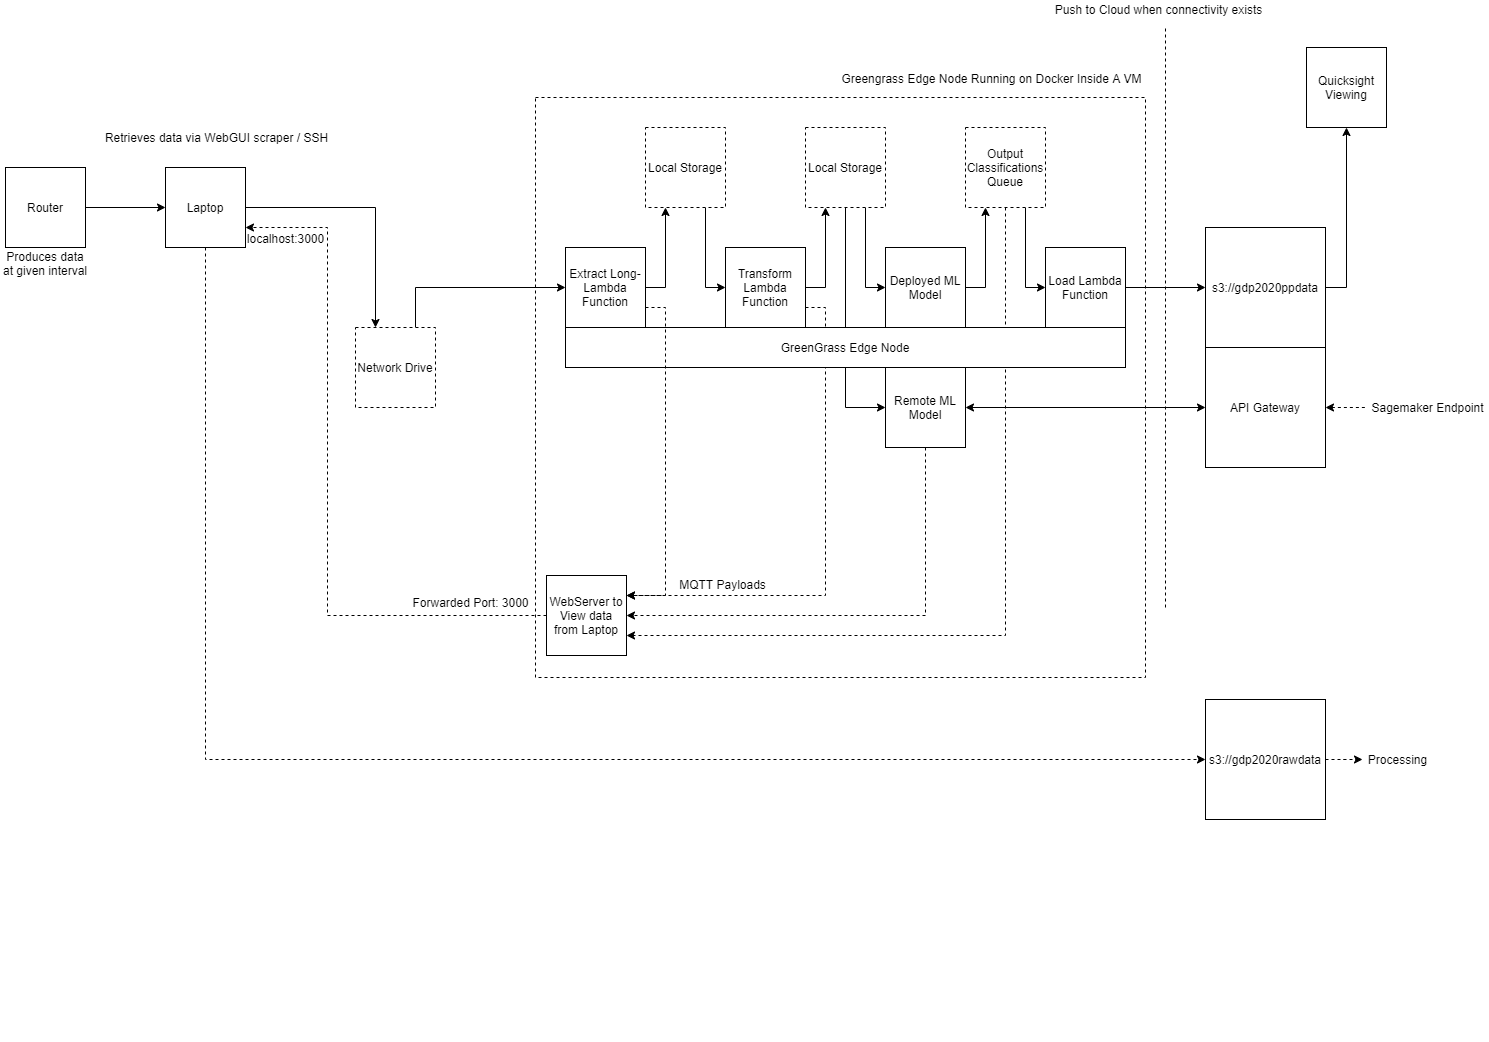
\includegraphics[width=1\linewidth]{pages/Chapter3/Chapter 3 images/greengrass_data_flow.png}
    \caption{The data flow within the Local Environment for Edge Computing - The full scale diagram can be seen in Appendix \ref{appendix:greengrass_design}}
    \label{fig:greengrass_edge_design}
\end{figure}

From the design in Figure \ref{fig:greengrass_edge_design}, we can see how the system will function for two out of the three pipelines discussed earlier. The first being the data is transported to the Edge only and the other for the data to be transported to the Cloud via the Edge.
\begin{enumerate}
    \item Data is collected from the router and stored in some (local) network data storage facility.
    \item This data is then retrieved by the Extract Lambda function running at the Edge and is stored locally.
    \item The Transform Lambda function will then begin the pre-processing of the data for usage and analysis.
    \item The Load Lambda function takes the pre-processed data and transfers it to the S3 Pre-Processed-Data bucket on the cloud.
    \item Pre-processed data is also taken to the ML-Inference Lambda function which uses an obtained ML Model from the Cloud for local classification of the data.
    \item Pre-processed data is used and a request is sent to the cloud for classification. Timings between Local ML-Classification and Remote ML-Classification can be compared.
    \item All data is sent to a local web-server showing all timings and classifications being made by the functions described.
    \item Timing data is also collected from the Laptop-to-Cloud pipeline scripts by another Lambda function and timings are shown in the Web Server. This also allows further comparison between the three pipeline options.
\end{enumerate}

The first point is discussed earlier in Section \ref{data_collection_design} about how data can be collected. Point two discusses the extract function. The laptop and the edge node share a network folder within the local environment. Data to be sent to the Edge Node will be placed into the shared folder by the laptop. In this case it is the raw data in the (.db) file format obtained from the router that is placed in the shared folder. The extract function will then take the database file and convert each data table within the database into it's own JSON file.

The third item discusses the transform function. This function \textit{compresses} all the JSON files that were extracted from the database file into a single array of all data elements corresponding to a single timestamp value as described in Section \ref{Section: JSON File Compression}. 

The fourth item describes the load function. Since edge nodes are often resource constrained in terms of hardware, either in processing power, memory available or data storage. It is often required to upload the data to the cloud upon good connectivity to ensure data is not lost and can be used for long-term analytics. The load function will then use API Gateway to securely send data to an S3 bucket to store the pre-processed data for any cloud-based processing and training of ML models. The load function allows for one of the two pipelines to be completed where data is transferred to the cloud via the edge node rather than directly from the laptop. The sixth item is also a part of this pipeline where data can be sent to a cloud endpoint where Sagemaker has deployed a ML model to classify data.

The fifth item discusses using a deployed ML Model that runs on the local edge node. This model is developed on the cloud using data that has been collected previously for training and verification. This model can then be deployed using Greengrass, where the model can be taken from any S3 bucket and then transported to the edge node. More about the model development is discussed in Section \ref{cloud_services}.

The seventh item in the list discusses the front-end of the Greengrass edge node. This is a custom solution to be able to view all the data in real-time for analysis or for any OTT application to be built on top of. The data is passed around from each Lambda function using MQTT packets. Each Lambda function can subscribes to a topic, e.g. 'server/extract/data', and on this topic another Lambda function can publish a message for it to be read by the subscribers. These data packets can all be seen by viewers on the cloud and so other services via AWS SNS (Simple Notification Service) are able to subscribe to these topics and then react accordingly especially for data viewing or analytics. For this project however, a custom GUI has been designed therefore a custom OTT Application could be implemented a top of it.

All three pipelines' data can be viewed at the Web Server and direct comparisons can be made of the timings of each function and help to evidence why deploying ML Models to edge is so advantageous to industry.

\subsection{AdvantEDGE}
AdvantEDGE is a Mobile Edge Emulation Platform (MEEP) that runs on Docker and Kubernetes. It is composed of micro-services that are packaged in Docker containers, interacting together to allow the deployment and edge scenario testing. AdvantEDGE provides an emulation environment that enables experimentation on the edge computing technologies, applications and services. The platform facilitates exploring edge deployment models and their impact on applications and services in short and agile iterations. The user is able to define a scenario that includes:
\begin{itemize}
    \item A network topology consisting of cloud, internet, general cellular operators, points of access (PoA), zones and edge/fog/user equipment (UE) application.
    \item Network characteristics for each of the elements set up including latency, latency variation (jitter), jitter distribution, packet loss and data throughput.
    \item Network and mobility events to change network characteristics and the location of UE and cloudlets during simulation run time. 
\end{itemize}

It allows the connection of the end points of the network simulation model to the real edge/fog/UE applications so that the performance which revolve around latency and data throughput can be captured especially in between the source and destination nodes. This enable the users to foresee and analyze the behavior and ability of the network model. With the third parties such as InfluxDB and Grafana in AdvantEDGE, the platform able to collect the measurements for graphing purpose and also support scripting for the network and mobility events. AdvantEDGE and instrumented clients load the data into InfluxDB time series database to stores the network and event measurements from deployed scenarios then display them through Grafana dashboards. Grafana dashboards were primarily used to monitor scenario execution and for demonstration purposes. This combination makes it a powerful platform for the edge network simulation.

\begin{figure}[ht]
    \centering
    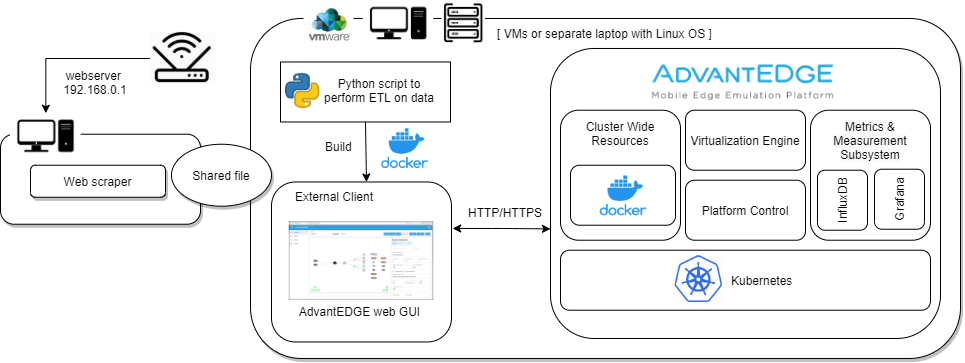
\includegraphics[width=1\linewidth]{pages/Chapter3/Chapter 3 images/System Diagram.png}
    \caption{The system diagram of edge application deployment to the AdvantEDGE - The full scale diagram can be seen in Appendix \ref{appendix:AdvantEDGE_edge_design}}
    \label{fig:AdvantEDGE_edge_design}
\end{figure}

Figure \ref{fig:AdvantEDGE_edge_design} shows the proposed system diagram of edge application deployment on the AdvantEDGE. The data collected from the router will be accessed by the VM through shared file, where Python scripts will extract data to convert from .db into JSON files. Then transform functions will compress these JSON files into one, before loading the JSON file into the ML model for evaluation. To be able to use the functionality of the Mobile Edge Emulation Platform, these Python applications will need to be built as Docker images before deploying them as a native edge application. A detailed step-by-step on installing AdvantEDGE can be found at \cite{kevin_2020}.

